\title{libSBOLj Tutorial}
\documentclass[10pt]{article}
\textwidth 6.5in
\textheight 9in
\oddsidemargin -0.2in
\topmargin -0.5in

\usepackage{graphicx,times,amsmath} % Add all your packages here
\usepackage[all]{xy}
\usepackage{multirow}
\usepackage{graphicx}
\usepackage{color}
\usepackage{tabularx}
\usepackage{url}
\usepackage{amsmath}
\usepackage{amssymb}
\usepackage{multirow}
\usepackage[noend,ruled,linesnumbered]{algorithm2e}
\usepackage[numbers, sort]{natbib}
\usepackage{listings}
\usepackage[svgnames]{xcolor}
%\usepackage{newtxtext}
\definecolor{javared}{rgb}{1,0,0} % for strings
\definecolor{javagreen}{rgb}{0.25,0.5,0.35} % comments
\definecolor{javapurple}{rgb}{0.5,0,0.35} % keywords
\definecolor{javadocblue}{rgb}{0.25,0.35,1} % javadoc
\lstdefinestyle{highlight} {
moredelim=[is][\bfseries\textcolor{javadocblue}]{<<>>}{>><<},
moredelim=[is][\itshape]{!!}{??}
}
\lstset{language=Java,
  keywordstyle=\color{javapurple}\bfseries,
  stringstyle=\color{javared},
  commentstyle=\color{javagreen},
  basicstyle=\tt\small,        % the size of the fonts that are used
                               % for the code
  style=highlight,
  breakatwhitespace=false,         % sets if automatic breaks should only happen at whitespace
  breaklines=true,                 % sets automatic line breaking                   % sets the caption-position to bottom
  extendedchars=true,              % lets you use non-ASCII characters; for 8-bits encodings only, does not work with UTF-8
  showspaces=false,                % show spaces everywhere adding particular underscores; it overrides 'showstringspaces'
  showstringspaces=false,          % underline spaces within strings only
  showtabs=false,                  % show tabs within strings adding particular underscores
  tabsize=2,                     % sets default tabsize to 2 spaces
  numbers=left,
  %frameround=ftff,
  frame=shadowbox,
  rulecolor=\color{black},
  rulesepcolor=\color{gray}
  }
\usepackage{hyperref}
\hypersetup{
    colorlinks=true,
    citecolor=teal,
    linkcolor=olive, % Internal links, those generated by cross-referenced elements    
    urlcolor=blue % Links to web sites
}
\newcommand{\sbol}[1]{\textbf{#1}}

\begin{document}
  \setlength{\parindent}{1em}
  \setlength{\parskip}{0em}
  \setlength{\parsep}{0em}

\section*{Modeling CRISPR repression using {\tt libSBOLj 2.0}}
We now describe the CRISPR-based repression module and how it can be modeled and encoded using the {\tt libSBOLj 2.0} library. We use bold font in the following text and figure captions to mark available data model in SBOL 2.0. 

\subsection*{CRISPR repression model}
First, consider the CRISPR-based Repression Template \textbf{ModuleDefinition} shown in the center of Figure \ref{SBOL2}. It provides a generic description of CRISPR-based repression behavior. Namely, it includes generic \emph{Cas9}, \emph{guide RNA} (gRNA), and \emph{target} DNA \textbf{FunctionalComponent} instances. It also includes a \emph{genetic production} \textbf{Interaction} that expresses a generic target gene product.  Finally, it includes a \emph{non-covalent binding} \textbf{Interaction} that forms the Cas9/gRNA complex (shown as dashed arrows), which in turn participates in an \emph{inhibition} \textbf{Interaction} to repress the target gene product production (shown with a tee-headed arrow). The CRISPR-based Repression Template is then instantiated to test a particular CRISPR-based repression device, CRPb, by the outer CRPb Characterization Circuit \textbf{ModuleDefinition}.  This outer characterization circuit includes gene \textbf{FunctionalComponents} to produce specific products (i.e., mKate, Gal4VP16, cas9m\_BFP, gRNA\_b, and EYFP), as well as \textbf{FunctionalComponents} for the products themselves.  Next, it includes \emph{genetic production} \textbf{Interactions} connecting the genes to their products, and it has a \emph{stimulation} \textbf{Interaction} that indicates that Gal4VP16 stimulates production of EYFP.  Finally, it uses \textbf{MapsTo} objects (shown as dashed lines) to connect the generic \textbf{FunctionalComponents} in the template to the specific objects in the outer \textbf{ModuleDefinition}.  For example, the outer module indicates that the target protein is EYFP, while the cas9\_gRNA complex is cas9m\_BFP\_gRNA\_b.

\begin{figure}[tbph]
\begin{center}
  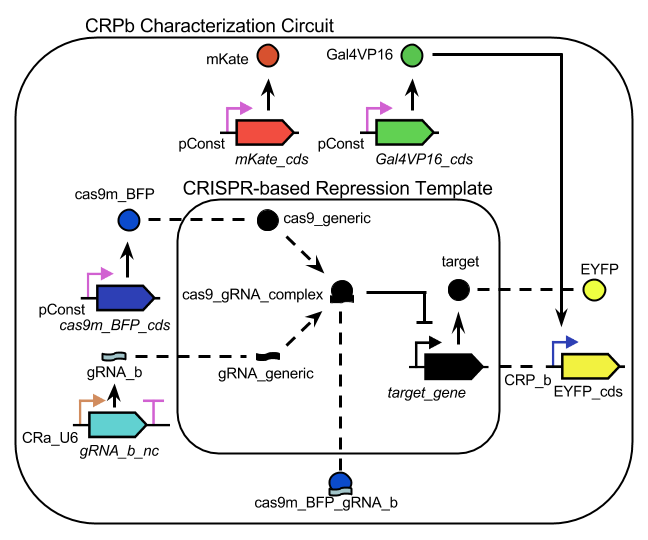
\includegraphics[width=0.95\textwidth]{figures/crispr_repression2} 
\end{center}
\caption{\label{SBOL2} Illustration of a hierarchical CRISPR-based repression module represented in SBOL 2.0 (adapted from Figure 1a in \cite{kiani2014crispr}). The CRISPR-based Repression Template \textbf{ModuleDefinition} describes a generic CRISPR repression circuit that combines a Cas9 protein with a gRNA to form a complex (represented by the dashed arrows) that represses a target gene (represented by the arrow with the tee arrowhead).  These relationships between these \textbf{FunctionalComponents} (instances of \textbf{ComponentDefinitions}) are represented in SBOL 2.0 using \textbf{Interactions}.  This \textbf{Module} is instantiated in the outer CRPb Characterization Circuit \textbf{ModuleDefinition} in order to specify the precise (including \textbf{Sequences} when provided) \textbf{FunctionalComponents}  used for each generic \textbf{FunctionalComponent}. The undirected dashed lines going into the template \textbf{Module} represent \textbf{MapsTo} objects that specify how specific \textbf{FunctionalComponents} replace the generic ones.}
\end{figure}

\subsection*{Encoding using {\tt libSBOLj 2.0}}
Program~\ref{JavaExample} illustrates the use of the {\tt libSBOLj 2.0} library using an excerpt of the Java code to express the CRISPR-based repressor design in SBOL 2.0. First, a new \textbf{SBOLDocument} is created (line 1), and is given a default URI prefix (line 2). At this point, \textbf{ComponentDefinition} and \textbf{Interaction} objects are also created for the CRISPR-based Repression Template \textbf{ModuleDefinition} (not shown).  Then, \textbf{Sequence} objects are created for those sequences provided in \cite{kiani2014crispr}.\footnote{Unfortunately, as usual, not all sequences are provided in the paper.} For example, to create the sequence for the CRP\_b promoter, we call the {\tt createSequence} method with the \emph{displayId} (CRP\_b\_seq), \emph{version} (1.0), the sequence, and the encoding used (line 3).  
Note that this method, as well as other create methods in the library, creates a \emph{compliant URI} that has the following form:
\begin{center}
http://$\langle$prefix$\rangle$/$\langle$displayId$\rangle$/$\langle$version$\rangle$
\end{center}
using the default URI prefix and provided \emph{displayId} and \emph{version}. The \emph{$\langle$prefix$\rangle$} represents a URI for a namespace (for example, {\tt www.sbols.org/CRISPR\_Example}). The author of a \textbf{TopLevel} object, such as the \textbf{Sequence} object we just created, should use a URI prefix that either they own or an organization of which they are a member owns. When using compliant URIs, the owner of a prefix must ensure that the URI of any unique \textbf{TopLevel} object that contains the prefix also contains a unique  \emph{$\langle$displayId$\rangle$} or \emph{$\langle$version$\rangle$} portion. Multiple versions of an SBOL object can exist and would have compliant URIs that contain identical prefixes and displayIds, but each of these URIs would need to end with a unique version. Lastly, the compliant URI of a non-\textbf{TopLevel} object is identical to that of its parent object, except that its displayId is inserted between its parent's displayId and version. This form of compliant URIs is chosen to be easy to read, facilitate debugging, and support a more efficient means of looking up objects and checking URI uniqueness. 

\begin{program*}[ht]
\begin{lstlisting}[language=java,style=highlight]
SBOLDocument doc = new SBOLDocument();
doc.setDefaultURIprefix("http://sbols.org/CRISPR_Example/");
doc.createSequence("CRP_b_seq", "1.0", "GCTCCGAATTTCTCGACAGATCTCATGTGAT...", !!Sequence??.<<>>IUPAC_DNA>><<); 
ComponentDefinition CRP_b = doc.createComponentDefinition("CRP_b", "1.0", !!ComponentDefinition??.<<>>DNA>><<);
CRP_b.addRole(!!SequenceOntology??.<<>>PROMOTER>><<);
CRP_b.addSequence("CRP_b_seq");
doc.createComponentDefinition("EYFP_cds", "1.0", !!ComponentDefinition??.<<>>DNA>><<).addRole(!!SequenceOntology??.<<>>CDS>><<);
ComponentDefinition EYFP_gene = doc.createComponentDefinition("EYFP_gene", "1.0", !!ComponentDefinition??.<<>>DNA>><<);
EYFP_gene.createSequenceConstraint("EYFP_gene_constraint", !!RestrictionType??.<<>>PRECEDES>><<, "CRP_b", "EYFP_cds");
doc.createComponentDefinition("Gal4VP16", "1.0", !!ComponentDefinition??.<<>>PROTEIN>><<);
ModuleDefinition CRPb_circuit = doc.createModuleDefinition("CRPb_characterization_circuit", "1.0");
Interaction EYFP_Activation = CRPb_circuit.createInteraction("EYFP_Activation", 
                                                             !!SystemsBiologyOntology??.<<>>STIMULATION>><<);
EYFP_Activation.createParticipation("GAL4VP16", "Gal4VP16").addRole(!!SystemsBiologyOntology??.<<>>STIMULATOR>><<);
EYFP_Activation.createParticipation("EYFP_gene", "EYFP_gene").addRole(!!SystemsBiologyOntology??.<<>>PROMOTER>><<);
Module Template_Module = CRPb_circuit.createModule("CRISPR_Template", "CRISPR_Template", "1.0");
Template_Module.createMapsTo("EYFP_gene_map", !!RefinementType??.<<>>USELOCAL>><<, "EYFP_gene", "target_gene");
\end{lstlisting}
\caption{\label{JavaExample}Fragments of Java code to produce part of the CRISPR Repression example using {\tt libSBOLj 2.0}.}
\end{program*}

Next, we create \textbf{ComponentDefinition} objects for each element in the module. For example, a \textbf{ComponentDefinition} of DNA type is created for the CRP\_b promoter (lines 4-6).  Note that by using compliant URIs, the sequence can be looked up using its \emph{displayId}, and since no version is provided, it is referenced by its \emph{persistentIdentity} URI (line 6). It is simply its URI without the version when using compliant URIs. The purpose of a persistent identity is to allow an object to refer to the latest version of another object using this URI. The latest version of an object is determined using \emph{semantic versioning} conventions (c.f., {\tt http://semver.org/}).

Next, we create two \textbf{ComponentDefinition} objects, one for the EYFP \emph{coding sequence} (CDS), and one for the EYFP gene (lines 7-8). We use a \textbf{SequenceConstraint} object (line 9) to indicate that the CRP\_b promoter precedes the EYFP CDS, because the sequence for the CDS has not been provided and thus cannot be given an exact \textbf{Range}. Finally, we create a protein type \textbf{ComponentDefinition} for the Gal4VP16 protein (line 10). After all the \textbf{ComponentDefinitions} are created, we create a \textbf{ModuleDefinition} object for the CRPb Characterization Circuit (line 11). 

Next, the \textbf{Interactions} between the components are specified using terms from the \emph{Systems Biology Ontology} (SBO) \cite{Courtot2011}.  One example \textbf{Interaction} is the stimulation of the \texttt{EYFP\_gene} by the Gal4VP16 protein (lines 12-14).  Now, the CRISPR-based Repression Template \textbf{Module} is instantiated and connected to the CRPb Characterization Circuit using \textbf{MapsTo} objects.  
For example, a \textbf{MapsTo} object is used to indicate that the \texttt{target\_gene} in the template should be refined to be the \texttt{EYFP\_gene} specified in the CRPb circuit (line 17).  

As we mentioned previously, the complete repression model is described in the ``RepressionModel.java'' under the libSBOLj examples directory. This example is self-contained in that you can run it to generate the RDF/XML output. Also, SBOL does not provide the specification of a mathematical model directly. It is possible, however, to generate a mathematical model using SBML~\cite{SBML} and the procedure described in~\cite{roehner2015generating}. Then, the SBOL document can reference this generated SBML model.



\section*{Other Methods in the API of {\tt libSBOj}}
So far, we have demonstrated how one can build the CRISPR-based repression module ~\cite{kiani2014crispr} using {\tt libSBOLj}. In this section, we present other major methods in the library's API. 

\subsection*{Retrieving an Existing Object}
Often, we need getter methods to retrieve a previously created object. You can easily do this by calling a ``get'' method in the \sbol{SBOLDocument} class to get back the \sbol{TopLevel} object you are looking for. For example, if we want to get the \lstinline+cas9_generic+ protein \sbol{ComponentDefinition} object, we can use the \lstinline+getComponentDefinition+ method (lines 1-4) shown below by providing the display ID and version of the object. If we want to get the latest version of a \sbol{TopLevel} object, we can pass \lstinline+null+ to its version field (lines 5-8), and the getter method will retrieve the object with the latest version. This is an implementation of the persistent identity feature. In our case, since we only have one version of the \lstinline+cas9_generic+ object, the two retrieved objects, namely \lstinline+cas9_generic1+ and \lstinline+cas9_generic2+, are identical, which can checked by calling the \lstinline+equals+ method (lines 9-11). In fact, they refer to the same object, i.e. \lstinline+cas9_generic+. The library provides \lstinline+equals+  method for every data model class, as well as the \sbol{SBOLDocument} class. To retrieve a non-\sbol{TopLevel} object, the getter method needs to be called on its immediate parent object. For example, line 12 below retrieves the \lstinline+gRNA_b_gene_constraint1+ from its parent \sbol{ComponentDefinition} \lstinline+gRNA_b_gene+. There is no need to provide the version here, because the child object's version is \emph{always} the same as its immediate parent's, under our compliant URI scheme.

\vspace{\abovedisplayskip}
\begin{minipage}{0.95\textwidth} 
\begin{lstlisting}
ComponentDefinition cas9_generic1 = doc.getComponentDefinition(
        "cas9_generic", 
        version
        );
ComponentDefinition cas9_generic2 = doc.getComponentDefinition(
        "cas9_generic", 
        null
        );
if (cas9_generic1.equals(cas9_generic2)) {
    System.out.println("Two Cas9 generic protein objects are equal.");
}
gRNA_b_gene.getSequenceConstraint("gRNA_b_gene_constraint1");
\end{lstlisting}
\end{minipage}

\subsection*{Manipulating Optional Fields}
For any optional field that is not a set or list, the library provides methods to set its value, unset its value to \lstinline+null+, and check its value. The only exceptions where these methods are not available are the following three fields in the \lstinline+Identified+ class: \lstinline+persistentIdentity+, \lstinline+displayId+, and
\lstinline+version+.  These fields cannot be edited, since they are crucial to maintaining
compliant SBOL objects (see Section~11.2 ``Compliant SBOL Objects'' of the~\href{http://sbolstandard.org/downloads/specification-data-model-2-0/}{Specification
  (Data Model 2.0)} for more details).  The example code below first sets the name of the \lstinline+CRISPR_Template+ \sbol{ModuleDefinition} with some garbage characters, it then unsets the name and rename it with a clear one. The code then sets the description of this object to the source of its bibliographic information. 

\vspace{\abovedisplayskip}
\begin{minipage}{0.95\textwidth} 
\begin{lstlisting}
CRISPR_Template.setName("C~R*I!S@P#R-based Repression Template");
if (CRISPR_Template.isSetName()) { // always true in this case
	CRISPR_Template.unsetName();
	CRISPR_Template.setName("CRISPR-based Repression Template");
}
CRISPR_Template.setDescription(
        "Authors: S. Kiani, J. Beal, M. Ebrahimkhani, J. Huh, R. Hall, Z. Xie, Y. Li, and R. Weiss," + 
        "Titel: Crispr transcriptional repression devices and layered circuits in mammalian cells," + 
        "Journal: Nature Methods, vol. 11, no. 7, pp. 723–726, 2014."
        );
\end{lstlisting}
\end{minipage}

For an optional field that is either a list or a set, the library provides methods for adding, removing, and checking if an element is contained in the list or set. One example we have seen several times so far is the call to the \lstinline+addRole+ method. Previously, we added the \lstinline+PROMOTER+ role, which is defined as \url{http://identifiers.org/so/SO:0000167}, to \lstinline+gRNA_b_gene+. The code below adds a second role \lstinline+gRNA_b_gene_role2+ to it first, it then checks the containment of this role before removing it. 

\vspace{\abovedisplayskip}
\begin{minipage}{0.95\textwidth} 
\begin{lstlisting}
URI gRNA_b_gene_role2 = URI.create("http://identifiers.org/so/SO:0000613"); 
gRNA_b_gene.addRole(gRNA_b_gene_role2);
if (gRNA_b_gene.containsRole(gRNA_b_gene_role2)) {
  gRNA_b_gene.removeRole(gRNA_b_gene_role2);
}
\end{lstlisting}
\end{minipage}

Fields that are a list or set of objects also include operations to clear, get, and set them.  The example code below removes all roles at once by calling \lstinline+clearRoles()+, gets the set of roles for the \lstinline+gRNA_b_gene+, and checks if it is empty.   Finally, it sets the entire set of roles (replacing any existing set) by calling \lstinline+setRoles(Set<URI> roles)+. At this point, \lstinline+gRNA_b_gene+ should only contain one role, which is \lstinline+PROMOTER+.

\vspace{\abovedisplayskip}
\begin{minipage}{0.95\textwidth} 
\begin{lstlisting}
gRNA_b_gene.clearRoles();
if (!gRNA_b_gene.getRoles().isEmpty()) {
  System.out.println("gRNA_b_gene set is not empty.");
}
gRNA_b_gene.setRoles(new HashSet<URI>(
        Arrays.asList(
        SequenceOntology.PROMOTER))
        );
 \end{lstlisting}
\end{minipage}

\subsection*{Creating and Editing References}
\sbol{TopLevel} objects can refer to other \sbol{TopLevel} objects.  For example, 
a \lstinline+ComponentDefinition+ object can refer to one or more sequences.  This reference is created by calling the \lstinline+addSequence(URI)+ method.  Methods available for manipulating references are similar to those for the optional fields. Previously, we added the \lstinline+CRP_b_seq+ \sbol{Sequence} to the \lstinline+CRP_b+ \sbol{ComponentDefinition}. The code below first clears all sequences associated with \lstinline+CRP_b+,  then adds the \lstinline+CRP_b_seq+ \sbol{Sequence} back. The last three lines will cause an exception to be thrown indicating that the sequence with the specified URI cannot be found in the \lstinline+doc+ \sbol{SBOLDocument} object. Note that since the ``complete'' flag is set to \lstinline+true+, the library verifies that all objects referenced are present in it.

\vspace{\abovedisplayskip}
\begin{minipage}{0.95\textwidth} 
\begin{lstlisting}
CRP_b.clearSequences();
CRP_b.addSequence("CRP_b_seq");
CRP_b.addSequence(
	URI.create("http://partsregistry.org/seq/partseq_154")
	);
\end{lstlisting}
\end{minipage}

\subsection*{Creating Annotations}
In order to allow representation of data that can not currently be represented
by the SBOL data model or data that are outside the scope of SBOL,
SBOL offers developers the ability to embed custom data as annotations
of SBOL objects and as generic top-level objects. These data are exchanged unmodified between
software tools that adopt {\tt libSBOLj 2.0}. 

Each object in SBOL 2.0 can be annotated by having any number of
\lstinline+Annotation+ objects that store data in the form of name/value 
property pairs. The name of an annotation must be a \lstinline+QName+
object, which is composed of a namespace, a
local name, and an optional prefix. The value of an annotation must contain a literal (i.e., a
\lstinline+String+, \lstinline+int+, \lstinline+double+,
\lstinline+boolean+), URI, or NestedAnnotations object. The code
snippet below creates an annotation for the \lstinline+pConst+ promoter. First, a new namespace is added to \lstinline+document+. It creates a short name ``pr'' for the \lstinline+prURI+
previously defined as the default URI prefix for this SBOL
document. This annotation is named ``pr:experience'', and is composed of
the \lstinline+prURI+ namespace, a local name ``experience'' and its prefix ``pr''.  It
contains a URI that can be resolved to the information web page
on the Parts Registry for the constitutive promoter `` J23119''.

\vspace{\abovedisplayskip}
\begin{minipage}{0.95\textwidth} 
\begin{lstlisting}
String prURI = "http://partsregistry.org"; 
String prPrefix = "pr";
doc.addNamespace(URI.create(prURI) , prPrefix);
ComponentDefinition pConst = doc.getComponentDefinition("pConst", version);
pConst.createAnnotation(
        new QName(prURI, "experience", prPrefix),
        URI.create("http://parts.igem.org/Part:BBa_J23119:Experience"));
\end{lstlisting}
\end{minipage}

\subsection*{Creating Generic TopLevel Object}
To embed custom data directly in an SBOL document, we can store them
using \lstinline+GenericTopLevel+ objects. The example code below first
creates such an object \lstinline+datasheet+, whose display ID is
``datasheet'' and version is ``1.1''. Its required RDF type property
is a \lstinline+QName+ object named
``myersLab:datasheet''. Then we set its name to
``Datasheet for Custom Parameters''. Custom data are encoded as annotations of this generic
top-level object. The first one is the characterization data with a
URI value that can be resolved to a location where measurement data
can be found. The next annotation stores the value of the
transcription rate, which is 0.75. The last three lines create
an annotation for \lstinline+TetR_promoter+ that refers to the
\lstinline+datasheet+ object.

\vspace{\abovedisplayskip}
\begin{minipage}{0.95\textwidth} 
\begin{lstlisting}
String myersLabURI = "http://www.async.ece.utah.edu";
String myersLabPrefix = "myersLab";	
GenericTopLevel datasheet=doc.createGenericTopLevel(
			"datasheet",
			"1.1",
      new QName(myersLabURI, "datasheet", myersLabPrefix));
datasheet.setName("Datasheet for Custom Parameters");		
datasheet.createAnnotation(
				new QName(myersLabURI, "characterizationData", myersLabPrefix), 
				URI.create(myersLabURI + "/measurement/Part:BBa_J23119:Experience"));				
datasheet.createAnnotation(
				new QName(myersLabURI, "transcriptionRate", myersLabPrefix), 
				0.75);
pConst.createAnnotation(
				new QName(myersLabURI, "datasheet", myersLabPrefix), 
				datasheet.getIdentity());
\end{lstlisting}
\end{minipage}

\subsection*{Creating and Editing Child Objects}
Certain classes in the SBOL 2.0 data model are allowed to own non-\sbol{TopLevel} child
objects that are also part of the data model. For example, all
\sbol{SequenceConstraints} we created previously are child objects of
their corresponding parent \sbol{ComponentDefinitions}, and all
\sbol{MapsTo} objects we created are child objects of their corresponding
parent \sbol{Modules}. Note that a child object can not exist on its
own, it therefore can only be created from its immediate parent
object. The library provides similar methods for retrieving,
removing and checking containment of child objects. Adding a child object to a parent
object is not directly available, due to our effort in maintaining
URI persistance between them. This, however, can be done by calling
the create method on its immediate parent, which adds the child object after its creation. 

\subsection*{Copying Objects}
The library can make copies of \sbol{TopLevel} objects using the \lstinline+createCopy+ methods.  There are several variations of this method. The \lstinline+createCopy(TopLevel)+ method makes an identical copy of its given \sbol{TopLevel} object. Note that this will cause an exception if it is copied into the same \sbol{SBOLDocument}, since it will not have a unique identity. Therefore, this method is meant to be used only when one wants to copy an object from one SBOL document to another. The \lstinline+createCopy(TopLevel, String)+ takes a \sbol{TopLevel} object to be copied and a new display ID, and it returns an identical copy with the display ID, and its own and its descendant's URI identities updated accordingly. There is a copy method that also takes a version field, and it returns a copy with the version, and its own and its descendant's URI identities updated accordingly.  Finally, a new URI prefix can also be provided, once again resulting in updated identities. The example below makes a copy of the
\lstinline+pConst+ promoter by calling \lstinline+createCopy+ with a new display ID, \lstinline+pConst_alt+. The identity URI for \lstinline+pConst_alt+ is changed to include the new display ID, and this change also percolates through the identity URIs for any of its descendent objects.  This example gives the new copy a sequence, but it keeps all other properties the same. 

\vspace{\abovedisplayskip}
\begin{minipage}{0.95\textwidth} 
\begin{lstlisting}
ComponentDefinition pConst_alt = (ComponentDefinition) doc.createCopy(pConst, "pConst_alt");
Sequence pConst_alt_seq = doc.createSequence(
        "pConst_alt_seq", 
        version, 
	"ttgacggctagctcagtcctaggtacagtgctagc",
	Sequence.IUPAC_DNA); 
pConst_alt.addSequence(pConst_alt_seq);
\end{lstlisting}
\end{minipage}

\subsection*{Serialization}
The library supports reading and writing data encoded in RDF/XML
format. We can produce a serialization output by
calling various write methods in the \sbol{SBOLWriter}
class. These methods write to either an output stream in the form of
Java OutputStream object or a file, some
of which are demonstrated below. The first method call produces an output
stream and the second stores the output to file
``RepressionModel.rdf''. Note that these two method calls do not
specify the output file type, and the library's default serialization
output format is RDF/XML.

\vspace{\abovedisplayskip}
\begin{minipage}{0.95\textwidth} 
\begin{lstlisting}
  SBOLWriter.write(doc,(System.out));
  SBOLWriter.write(doc, "RepressionModel.rdf");
\end{lstlisting}
\end{minipage}

Reading of a file or an input stream in the form of Java InputStream
object is supported by similar read methods in the \sbol{SBOLReader}
class. The default input format for any of these read methods is also
RDF/XML. The method below first writes the \sbol{SBOLDocument}
``\lstinline+doc+'' to a Java \lstinline+ByteArrayOutputStream+,
and then reads it back to a new \sbol{SBOLDocument} object.

\begin{minipage}{0.95\textwidth} 
\begin{lstlisting}
public static SBOLDocument writeThenRead(SBOLDocument doc)
	               throws SBOLValidationException, IOException, XMLStreamException, FactoryConfigurationError, CoreIoException
{
  ByteArrayOutputStream out = new ByteArrayOutputStream();
  SBOLWriter.write(doc, out);
  return SBOLReader.read(new ByteArrayInputStream(out.toByteArray()));
}
\end{lstlisting}
\end{minipage}

% The RDF serialization for the SBOLDocument object created in this
% tutorial is shown below. Note that we only show the beginning of the
% actual sequences for \lstinline+seq_K137046+ and
% \lstinline+partseq_153+ in the serialization output below. Actual
% serialization includes the complete sequences.


\bibliographystyle{ieeetr}
\bibliography{top}


\end{document}
